\chapter{\Large Iteración II: “Información contextual y envió de alertas de seguridad”}
\label{iteracion2}
    Partiendo de la topología definida en la Figura \ref{fig:iter1_ver_RF1_RF2} de Iteración I, se procedió a verificar los requerimientos de prioridad media. Para ello se siguió con la misma metodología de prueba, que consistió en dos acciones ofensivas: un escaneo de puertos y un ataque de inyeccion SQL, ambos desde una terminal dentro de la Dependencia 1 a un activo ubicado dentro del datacenter llamado Servidor 1.
    \begin{section}{Verificación de RF2: Recolección de información contextual}
    La información contextual de un activo de información está constituida por todos aquellos datos que reflejan, en un momento particular, el estado del sistema. Entre los ejemplos se encuentran los logs de las peticiones recibidas, el estado de los servicios habilitados, la conexión a la red, parámetros de uso de hardware tales como el nivel de ocupación de disco, temperatura, uso de la memoria RAM, entre otros. Una anomalía en estos datos es útil para indicar que algo puede estar ocurriendo, tal como una acción ofensiva encubierta en operaciones habilitadas. Por ejemplo, un ataque DDoS implica el aumento exponencial de la frecuencia normal de transacciones. En el caso de un ataque no detectado por un IDS, estos datos sirven para alertar de que una posible acción ofensiva está teniendo lugar. \par
    Con el objetivo de recibir esta información, el servidor Master de Security Onion recolectó logs provenientes de servicios de “log shipping” (proceso de automatización del respaldo de archivos de logs de transacciones). Para este proyecto se optó por Filebeat. Este es un servicio que permite enviar información a Logstash desde múltiples directorios. El proceso comienza cuando el servicio lee línea por línea los archivos de entrada en un activo y envía los logs de la misma manera a Logstash (servidor Master). Este los recibe en su puerto 5044 por defecto, posteriormente puede filtrarlos para separar los campos de los logs o bien almacenarlos sin filtrar. \par
    La experiencia inició con el envío de los logs del estado de las aplicaciones de un servidor disponible en la organización, mediante Filebeat, a Logstash y sin un procesamiento posterior. Esto generó que ElastAlert no pudiera realizar una correlación al no identificar información clave, como la que se encuentra en los campos de puertos y direcciones IP de origen y destino, estampas de tiempo, tipo de peticiones, etc. Posteriormente se utilizó el plugin Grok \cite{grok} para filtrar los logs que estaba recibiendo Logstash antes de almacenarlos, con el fin de realizar detecciones basadas en correlaciones utilizando ElastAlert.\par
    Como se observa en la Figura \ref{fig:figura_iter2_ataque}, se realizó el envío de logs del Servidor 1 (que se encuentra conectado al Switch 3) mediante Filebeat al nodo Master que se encuentra conectado al Switch 4. Estos logs de accesos contenían información de un servidor web Apache, incluyendo consultas realizadas, métodos y otros metadatos de interés. Esta información resultó útil para identificar un ataque de aplicación web, de estilo “inyección SQL”, que fue realizado utilizando herramientas como “sqlmap” \cite{sqlmap}, desarrolladas en Python 3.5. Este tipo de ataque consiste en introducir, de manera iterativa, comandos SQL en un formulario web con el objetivo de lograr recabar información de las bases de datos del Servidor 1 (víctima), modificar e incluso eliminar dicha base de datos. El comando utilizado en sqlmap fue:
    \begin{verbatim}
        python sqlmap.py -u "http://IP_VICTIMA/login/index.php?id=101" --batch
    \end{verbatim} 
    donde los flags significan:
    \begin{itemize}
    \item \begin{verbatim}
        -u
    \end{verbatim}
     parámetro para especificar una URL.
    \item \begin{verbatim}
        "http://IP_victima/path/al/formulario?etc"
    \end{verbatim} 
    es el campo que contiene la dirección de un formulario en la página web víctima.
    \item \begin{verbatim}
        --batch
    \end{verbatim}
     es un switch que sirve para elegir la opción por defecto en paginas donde hay múltiples parámetros. La consecuencia de elegir la opción por defecto es que ahorra tiempo al evitar una elección del usuario.
    \end{itemize}
    \begin{figure}[H]
    \centering
    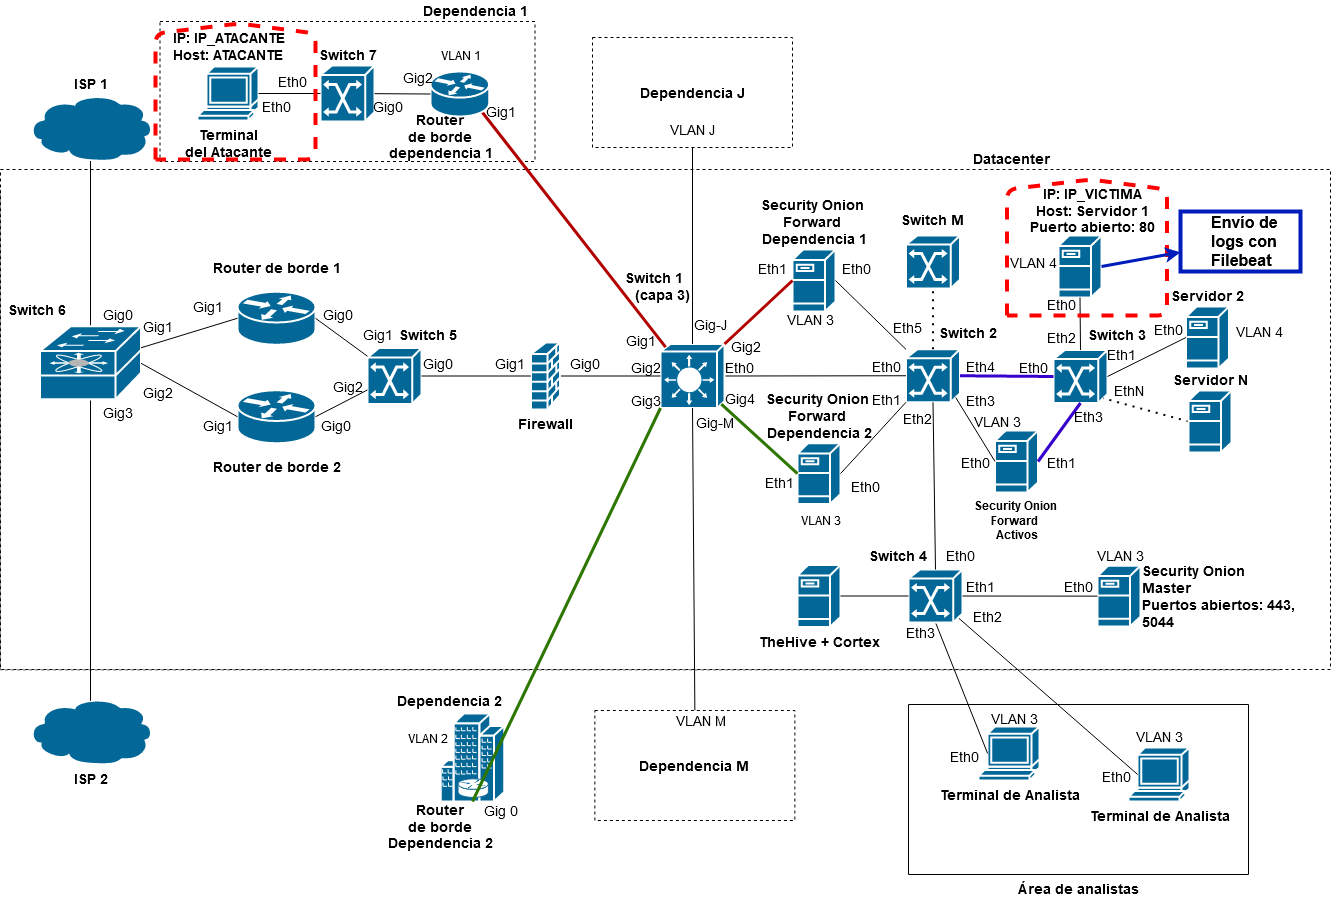
\includegraphics[width=1\textwidth]{./iteracion_2_imagenes/Topologia de despliegue descentralizada RF2, RF6 y RF4-FILEBEAT.png}
    \caption{Topología distribuida para la verificación de RF2, RF6 y RF4}
    \label{fig:figura_iter2_ataque}
    \end{figure}
    \FloatBarrier

    En la Figura \ref{fig:iter2_logs_crudos} se puede observar el almacenamiento de registros sin filtrar, con esto queda demostrado el cumplimiento del requerimiento funcional 2.
    \begin{figure}[H]
    \centering
    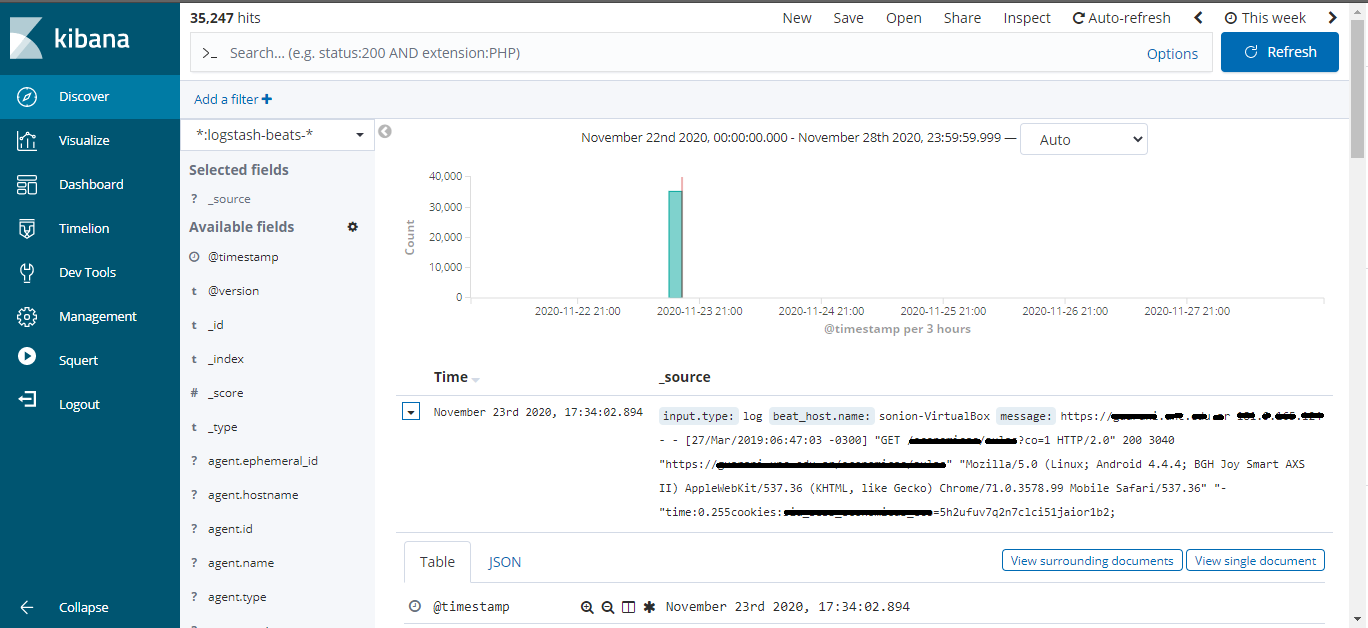
\includegraphics[width=1\textwidth]{./iteracion_2_imagenes/1_kibana_logs_1EDITADA.png}
    \caption{Almacenamiento de logs sin procesar}
    \label{fig:iter2_logs_crudos}
    \end{figure}
    \FloatBarrier
    Posteriormente se repitió la experiencia pero esta vez los logs que se recibían en Logstash eran procesados utilizando Grok. Esto permitió generar información estructurada capaz de ser consultada. \par
    En la Figura \ref{fig:figura_squert-sql} se pudo comprobar que el ataque de inyección SQL fue detectado en Squert.
    \begin{figure}[H]
    \centering
    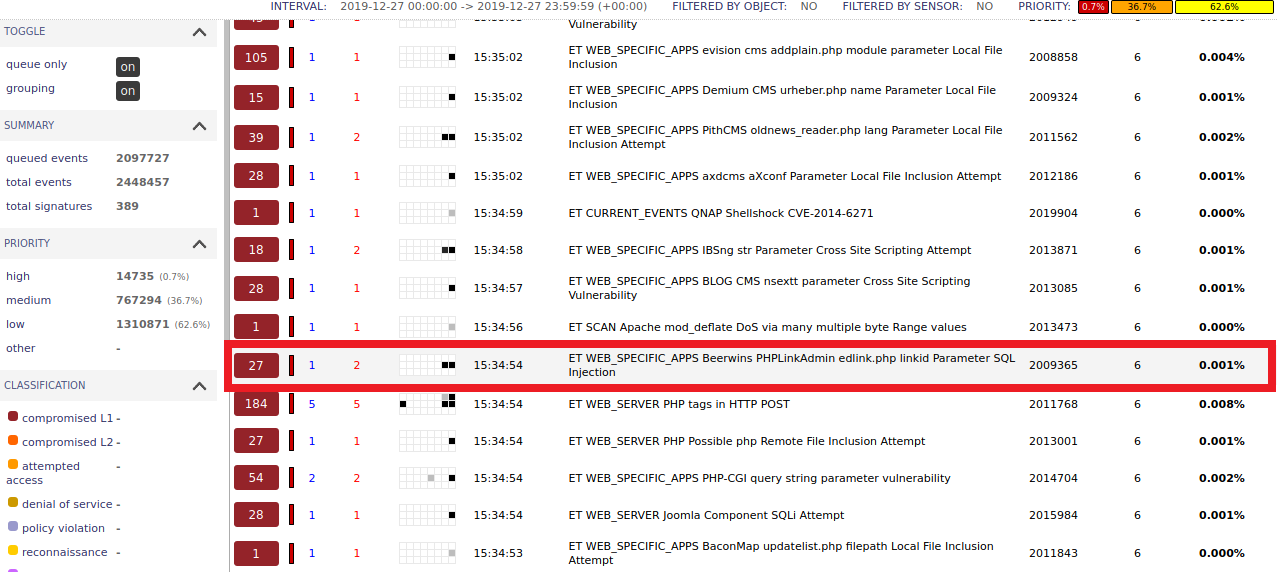
\includegraphics[width=0.7\textwidth]{./iteracion_2_imagenes/squert-sql-injection.png}
    \caption{Detección de un ataque de inyección SQL en el panel de Squert}
    \label{fig:figura_squert-sql}
    \end{figure}
    Los resultados en Kibana se ven en la Figura 6.3, donde se registraron las direcciones IP del Servidor 1 (víctima) y la del atacante. \par
    \begin{figure}[H]
    \centering
    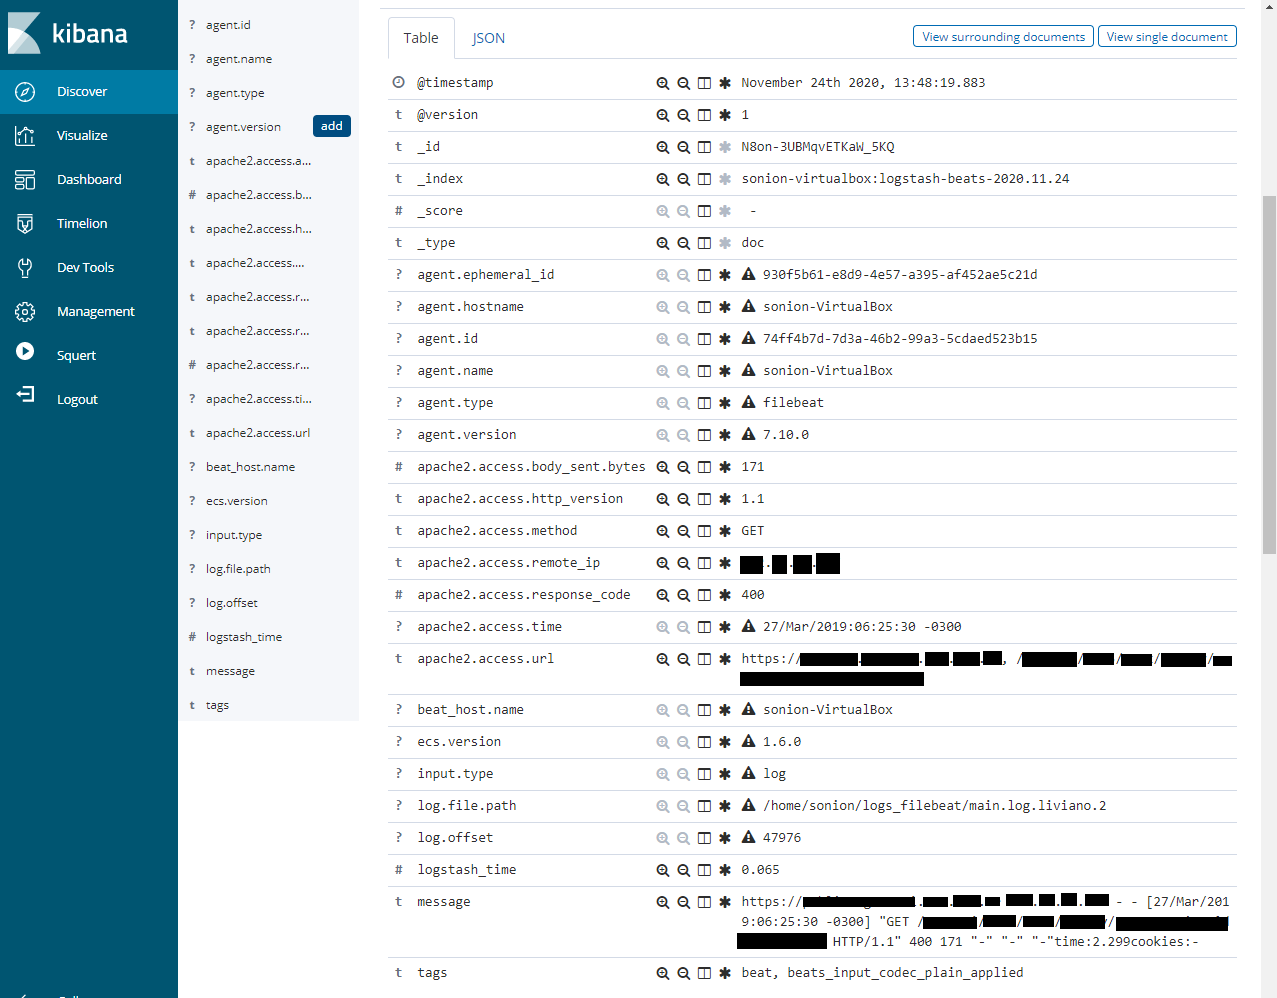
\includegraphics[width=1\textwidth]{./iteracion_2_imagenes/kibana_logs_parseados_2EDITADO.png}
    \caption{Almacenamiento de logs procesados por Logstash}
    \label{fig:iter2_logs_filtrados}
    \end{figure}
    \FloatBarrier
    Es importante mencionar que la información almacenada en Elasticsearch, es consultada constantemente por ElastAlert. Este último componente es el encargado de correlacionar los campos de los logs y enviar notificaciones.
    \end{section}
    \pagebreak
    
    \begin{section}{Verificación de RF6 y RF4: implementación de un sistema de correlación y envió de alertas de seguridad}
    El envío de alertas de seguridad y la notificación a los responsables de los activos que se ven afectados, fue realizado por ElastAlert. Este permite correlacionar la información presente en los campos de logs guardados en Elasticsearch, así como enviar notificaciones cuando se produce la detección de incidentes. \par
    
    ElastAlert es un framework que detecta patrones en los datos consultados, como anomalías, picos, etc. Como se mencionó en la sección \ref{seccion4-5}, basa su funcionamiento en dos componentes: reglas y alertas. \par
   
    Las alertas consisten en mensajes que permiten notificar a un usuario final o a otro sistema, sobre un evento de seguridad. Para esta prueba se realizó otro escaneo de puertos desde el “atacante” ubicado en la Dependencia 1 dirigido al Sevidor 1 (víctima), ubicado en el datacenter. Para esto se configuro a ElastAlert para que notifique por correo electrónico en el caso de detectar algún tipo de ataque de categoría “scan”.\par
    
    En la Figura \ref{fig:iter2_diagrama_envio_alertas} se observa un diagrama de secuencia del envío de una alerta. Esta comienza cuando los logs que llegan a Logstash son filtrados y enviados de forma estructurada (JSON) al puerto 9200 de Elastisearch. ElastAlert, por otro lado, realiza consultas periódicas a la base de datos mencionada. Cuando ElastAlert recibe una respuesta a su petición, procede a buscar patrones que se puedan identificar en los logs recibidos. \par
    
    Independientemente de la coincidencia o no de algún patrón, ElastAlert vuelve a consultar a Elasticsearch por otros logs y procede a repetir el procedimiento descrito, mientras este activo como servicio. En el caso de encontrar un patrón en los datos recibidos, se enviará una notificación a los responsables del activo afectado.\par
    \begin{figure}[H]
    \centering       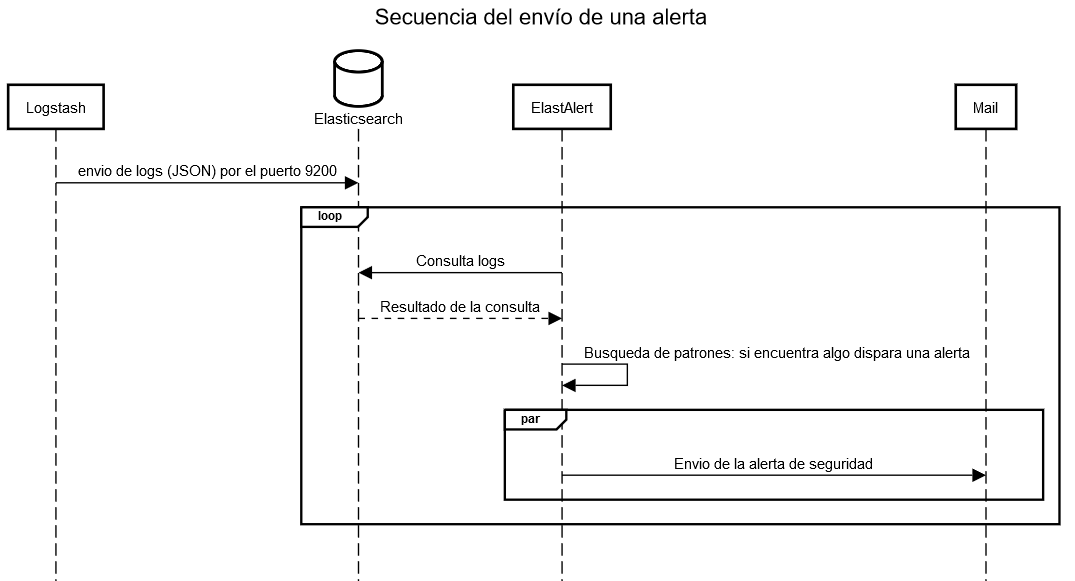
\includegraphics[width=1\textwidth]{./iteracion_2_imagenes/2-diagrama-de-secuencia-envio-alerta.png}
    \caption{Diagrama de secuencia del envío de una alerta}
    \label{fig:iter2_diagrama_envio_alertas}
    \end{figure}
    En la Figura \ref{fig:iter2_notificacion_alertas} se observa el correo electrónico recibido cuando se disparó una alerta por el ataque de reconocimiento. Con esto se verificaron RF4 y RF6.\par
    \begin{figure}[H]
    \centering       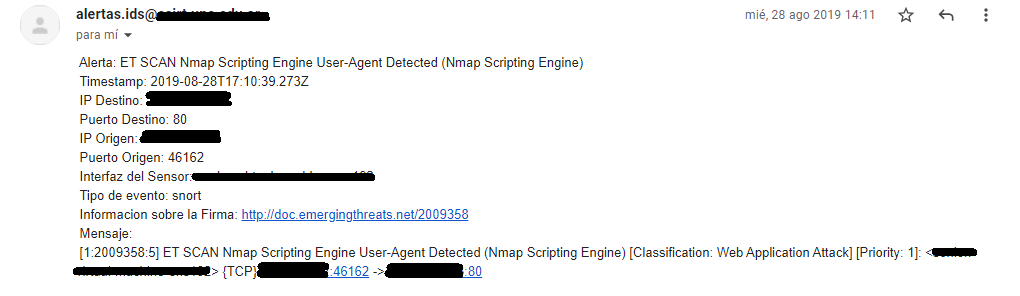
\includegraphics[width=1\textwidth]{./iteracion_2_imagenes/notificacion_alertas_1EDITADO.png}
    \caption{Notificación recibida debido a una alerta por reconocimiento de puertos}
    \label{fig:iter2_notificacion_alertas}
    \end{figure}
    
    \end{section}